%%%%%%%%%%%%%%%%%%%%%%%%%%%%%%%%%%%%%%%%%
% KOMA-Script Presentation
% LaTeX Template
% Version 1.0 (3/3/13)
%
% This template has been downloaded from:
% http://www.LaTeXTemplates.com
%
% Original Authors:
% Marius Hofert (marius.hofert@math.ethz.ch)
% Markus Kohm (komascript@gmx.info)
% Described in the PracTeX Journal, 2010, No. 2
%
% License:
% CC BY-NC-SA 3.0 (http://creativecommons.org/licenses/by-nc-sa/3.0/)
%
%%%%%%%%%%%%%%%%%%%%%%%%%%%%%%%%%%%%%%%%%

%----------------------------------------------------------------------------------------
%	PACKAGES AND OTHER DOCUMENT CONFIGURATIONS
%----------------------------------------------------------------------------------------

\documentclass[
paper=128mm:96mm, % The same paper size as used in the beamer class
fontsize=11pt, % Font size
pagesize, % Write page size to dvi or pdf
parskip=half-, % Paragraphs separated by half a line
]{scrartcl} % KOMA script (article)
\usepackage[spanish]{babel}
\selectlanguage{spanish}
\usepackage[utf8]{inputenc}
\linespread{1.12} % Increase line spacing for readability

%------------------------------------------------
% Colors
\usepackage{xcolor}	 % Required for custom colors
% Define a few colors for making text stand out within the presentation
\definecolor{mygreen}{RGB}{44,85,17}
\definecolor{myblue}{RGB}{34,31,217}
\definecolor{mybrown}{RGB}{194,164,113}
\definecolor{myred}{RGB}{255,66,56}
% Use these colors within the presentation by enclosing text in the commands below
\newcommand*{\mygreen}[1]{\textcolor{mygreen}{#1}}
\newcommand*{\myblue}[1]{\textcolor{myblue}{#1}}
\newcommand*{\mybrown}[1]{\textcolor{mybrown}{#1}}
\newcommand*{\myred}[1]{\textcolor{myred}{#1}}
%------------------------------------------------

%------------------------------------------------
% Margins
\usepackage[ % Page margins settings
includeheadfoot,
top=3.5mm,
bottom=3.5mm,
left=5.5mm,
right=5.5mm,
headsep=6.5mm,
footskip=8.5mm
]{geometry}
%------------------------------------------------

%------------------------------------------------
% Fonts
\usepackage[T1]{fontenc}	 % For correct hyphenation and T1 encoding
\usepackage{lmodern} % Default font: latin modern font
%\usepackage{fourier} % Alternative font: utopia
%\usepackage{charter} % Alternative font: low-resolution roman font
\renewcommand{\familydefault}{\sfdefault} % Sans serif - this may need to be commented to see the alternative fonts
%------------------------------------------------

%------------------------------------------------
% Various required packages
\usepackage{amsthm} % Required for theorem environments
\usepackage{bm} % Required for bold math symbols (used in the footer of the slides)
\usepackage{graphicx} % Required for including images in figures
\usepackage{tikz} % Required for colored boxes
\usepackage{booktabs} % Required for horizontal rules in tables
\usepackage{multicol} % Required for creating multiple columns in slides
\usepackage{lastpage} % For printing the total number of pages at the bottom of each slide
\usepackage{microtype} % Better typography
\usepackage{tocstyle} % Required for customizing the table of contents
\usepackage{verbatim}  % Needed for the "comment" environment to make LaTeX comments
%------------------------------------------------

%------------------------------------------------
% Slide layout configuration
\usepackage{scrpage2} % Required for customization of the header and footer
\pagestyle{scrheadings} % Activates the pagestyle from scrpage2 for custom headers and footers
\clearscrheadfoot % Remove the default header and footer
\setkomafont{pageheadfoot}{\normalfont\color{black}\sffamily} % Font settings for the header and footer

% Sets vertical centering of slide contents with increased space between paragraphs/lists
\makeatletter
\renewcommand*{\@textbottom}{\vskip \z@ \@plus 1fil}
\newcommand*{\@texttop}{\vskip \z@ \@plus .5fil}
\addtolength{\parskip}{\z@\@plus .25fil}
\makeatother

% Remove page numbers and the dots leading to them from the outline slide
\makeatletter
\newtocstyle[noonewithdot]{nodotnopagenumber}{\settocfeature{pagenumberbox}{\@gobble}}
\makeatother
\usetocstyle{nodotnopagenumber}

\AtBeginDocument{\renewcaptionname{spanish}{\contentsname}{\Large Índice}} % Change the name of the table of contents
%------------------------------------------------

%------------------------------------------------
% Header configuration - if you don't want a header remove this block
\ihead{
\hspace{-2mm}
\begin{tikzpicture}[remember picture,overlay]
\node [xshift=\paperwidth/2,yshift=-\headheight] (mybar) at (current page.north west)[rectangle,fill,inner sep=0pt,minimum width=\paperwidth,minimum height=2\headheight,top color=mygreen!64,bottom color=mygreen]{}; % Colored bar
\node[below of=mybar,yshift=3.3mm,rectangle,shade,inner sep=0pt,minimum width=128mm,minimum height =1.5mm,top color=black!50,bottom color=white]{}; % Shadow under the colored bar
shadow
\end{tikzpicture}
\color{white}\runninghead} % Header text defined by the \runninghead command below and colored white for contrast
%------------------------------------------------

%------------------------------------------------
% Footer configuration
\newlength{\footheight}
\setlength{\footheight}{8mm} % Height of the footer
\addtokomafont{pagefoot}{\footnotesize} % Small font size for the footnote

\ifoot{% Left side
\hspace{-2mm}
\begin{tikzpicture}[remember picture,overlay]
\node [xshift=\paperwidth/2,yshift=\footheight] at (current page.south west)[rectangle,fill,inner sep=0pt,minimum width=\paperwidth,minimum height=3pt,top color=mygreen,bottom color=mygreen]{}; % Green bar
\end{tikzpicture}
\myauthor\ \raisebox{0.2mm}{$\bm{\vert}$}\ \myuni % Left side text
}

\ofoot[\pagemark/\pageref{LastPage}\hspace{-2mm}]{\pagemark/\pageref{LastPage}\hspace{-2mm}} % Right side
%------------------------------------------------

%------------------------------------------------
% Section spacing - deeper section titles are given less space due to lesser importance
\usepackage{titlesec} % Required for customizing section spacing
\titlespacing{\section}{0mm}{0mm}{0mm} % Lengths are: left, before, after
\titlespacing{\subsection}{0mm}{0mm}{-1mm} % Lengths are: left, before, after
\titlespacing{\subsubsection}{0mm}{0mm}{-2mm} % Lengths are: left, before, after
\setcounter{secnumdepth}{0} % How deep sections are numbered, set to no numbering by default - change to 1 for numbering sections, 2 for numbering sections and subsections, etc
%------------------------------------------------

%------------------------------------------------
% Theorem style
\newtheoremstyle{mythmstyle} % Defines a new theorem style used in this template
{0.5em} % Space above
{0.5em} % Space below
{} % Body font
{} % Indent amount
{\sffamily\bfseries} % Head font
{} % Punctuation after head
{\newline} % Space after head
{\thmname{#1}\ \thmnote{(#3)}} % Head spec
	
\theoremstyle{mythmstyle} % Change the default style of the theorem to the one defined above
\newtheorem{theorem}{Theorem}[section] % Label for theorems
\newtheorem{remark}[theorem]{Remark} % Label for remarks
\newtheorem{algorithm}[theorem]{Algorithm} % Label for algorithms
\makeatletter % Correct qed adjustment
%------------------------------------------------

%------------------------------------------------
% The code for the box which can be used to highlight an element of a slide (such as a theorem)
\newcommand*{\mybox}[2]{ % The box takes two arguments: width and content
\par\noindent
\begin{tikzpicture}[mynodestyle/.style={rectangle,draw=mygreen,thick,inner sep=2mm,text justified,top color=white,bottom color=white,above}]\node[mynodestyle,at={(0.5*#1+2mm+0.4pt,0)}]{ % Box formatting
\begin{minipage}[t]{#1}
#2
\end{minipage}
};
\end{tikzpicture}
\par\vspace{-1.3em}}
%------------------------------------------------

%----------------------------------------------------------------------------------------
%	PRESENTATION INFORMATION
%----------------------------------------------------------------------------------------

\newcommand*{\mytitle}{Adaptabilidad al contexto en aplicaciones web desarrolladas con continuations} % Title
\newcommand*{\runninghead}{Adaptabilidad en aplicaciones web desarrolladas con continuations} % Running head displayed on almost all slides
\newcommand*{\myauthor}{Eloy Adonis Colell} % Presenters name(s)
\newcommand*{\mydate}{\today} % Presentation date
\newcommand*{\myuni}{Universidad Nacional de Luján} % University or department

%----------------------------------------------------------------------------------------

\begin{document}

%----------------------------------------------------------------------------------------
%	TITLE SLIDE
%----------------------------------------------------------------------------------------

% Title slide - you may have to tweak a few of the numbers if you wish to make changes to the layout
\thispagestyle{empty} % No slide header and footer
\begin{tikzpicture}[remember picture,overlay] % Background box
\node [xshift=\paperwidth/2,yshift=\paperheight/2] at (current page.south west)[rectangle,fill,inner sep=0pt,minimum width=\paperwidth,minimum height=\paperheight/3,top color=mygreen,bottom color=mygreen]{}; % Change the height of the box, its colors and position on the page here
\end{tikzpicture}
% Text within the box
\begin{flushright}
\vspace{0.6cm}
\color{white}\sffamily
{\bfseries\Large\mytitle\par} % Title
\vspace{0.5cm}
\normalsize
\myauthor\par % Author name
\mydate\par % Date
\vfill
\end{flushright}

\clearpage

%----------------------------------------------------------------------------------------
%	TABLE OF CONTENTS
%----------------------------------------------------------------------------------------

%\thispagestyle{empty} % No slide header and footer

%\small\tableofcontents % Change the font size and print the table of contents - it may be useful to shrink the font size further if the presentation is full of sections
% To exclude sections/subsections from the table of contents, put an asterisk after \(sub)section like so: \section*{Section Name}

%\clearpage

%----------------------------------------------------------------------------------------
%	PRESENTATION SLIDES
%----------------------------------------------------------------------------------------

\section{Combinar}

\begin{itemize}
	\item Aplicaciones web desarrolladas con Continuations.
	\item Adaptabilidad al Contexto.
\end{itemize}

\clearpage

%\section{Aplicaciones web}

%\begin{itemize}
%\item Son la evolución de las páginas web.
%\item Modifican su contenido a partir de la interacción con el usuario.
%\item Permiten la interacción entre usuarios.
%\end{itemize}

%\subsection{Utilizan frameworks basados en...}
%\begin{itemize}
%\item Model View Controller\cite{Gamma95}
%\item Continuations\cite{Ducasse04}
%\item otros
%\end{itemize}

%\clearpage

%\subsection{Estructura}
%\begin{figure}[ht!]
%\centering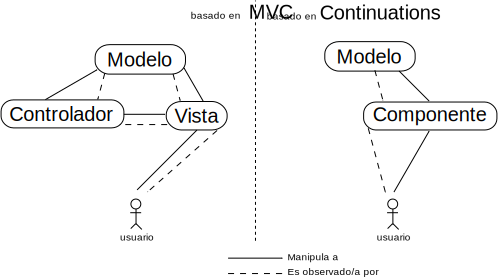
\includegraphics[width=0.9\linewidth]{Figures/MVCContinuations}
%\end{figure}

%\clearpage


\subsection{Aplicaciones web basadas en Continuations}

\begin{figure}[ht!]
\centering
Delegan el control de la pila de ejecución al procedimiento que será inmediatamente ejecutado (ver \textbf{Seaside}).
\end{figure}

\clearpage


%\subsection{Seaside como framework de Continuations}

%Existen 2 tipos de componentes:
%\begin{description}
%\item[WATask] Describen un \textbf{flujo de control}.
%\item[WAComponent] Describen un \textbf{flujo de control} y la \textbf{apariencia} de una porcion de la página web.
%\end{description}

%\clearpage

\subsection{Estructura de una aplicación que utiliza Seaside}

\begin{figure}[ht!]
\centering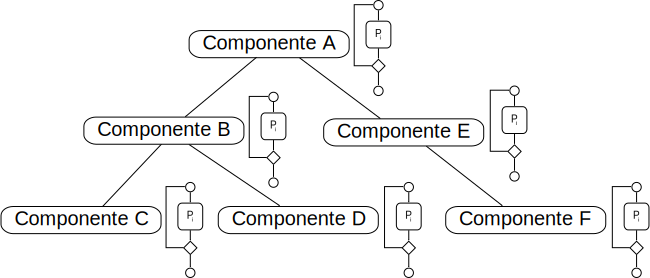
\includegraphics[width=0.8\linewidth]{Figures/Seaside}
\end{figure}

\clearpage

%\begin{figure}
%\centering
%¿Como se utiliza la técnica de \emph{Continuations}?
%\end{figure}

%\clearpage

%Se proveen 2 métodos para simplificar su uso dentro de una aplicación:
%\begin{description}
%\item[\#call:] Delega el control a otro componente.
%\item[\#answer:] Devuelve el control que le cedieron.
%\end{description}

%\clearpage


\section{Adaptabilidad al contexto}

%\begin{figure}[ht!]
%\centering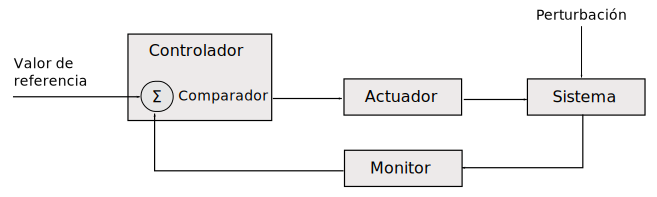
\includegraphics[width=0.8\linewidth]{../doc/Figures/FeedbackControlSystem}
%\end{figure}

%\begin{figure}[ht!]
%\small
%\textbf{Sistemas Adaptativos} + información externa = adaptación al contexto \\
%Sensibilidad al contexto = \textbf{adaptación al contexto} + evolución automática
%\end{figure}

%\clearpage

\subsection{¿Que significa Contexto?}
\begin{description}
\item[Dey\cite{Dey01}] Es cualquier información que pueda ser usada para caracterizar la situación de una entidad. Una entidad es una persona, un lugar, o un objeto que es considerado relevante para la interacción entre un usuario y una aplicación; incluyendo al mismo usuario y/o la misma aplicación dentro de los objetos posibles.
%\item[Dourish\cite{Dourish04}] Es un concepto de lo que se mantiene al margen, y se disuelve cuando uno intenta definirlo.
\end{description}

\clearpage

Según Efstratiou\cite{Efstratiou04}:

Las \textbf{aplicaciones adaptativas sensibles al contexto} son las que modifican su comportamiento (se adaptan) de acuerdo a los cambios en el contexto de la aplicación.

\begin{figure}[ht!]
\centering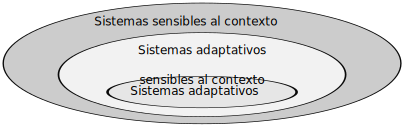
\includegraphics[width=0.8\linewidth]{../doc/Figures/ContextAwareSystems}
\end{figure}

\clearpage

%\begin{figure}
%\centering
%Los sistemas sensibles al contexto, incluyen tanto la \textbf{adaptación} como el análisis de la \textbf{evolución} del contexto.
%\end{figure}
%
%\clearpage


\section{¿Cuál es el problema?}

\begin{itemize}
\item Privacidad del usuario
\item Transacciones con adaptación al contexto
\end{itemize}

\clearpage

\subsection{Privacidad del usuario}

\begin{description}
\item[Aplicaciones web] Se ejecutan encapsuladas en el navegador web para proveer de cierta seguridad y privacidad al usuario.
\item[Sensibilidad al contexto] Necesitan el acceso a la información privada del usuario y a un conjunto de sus sensores, con el fin de identificar el contexto (o entorno) de forma automática y promocionar adaptaciones que simplifiquen la actividad cotidiana del usuario.
\end{description}

\clearpage

\subsection{Transacciones con adaptación al contexto}

En las \textbf{aplicaciones adaptativas} la persistencia de la información ocurre de forma acumulativa (se memoriza el progreso de los estados y de la adaptación a través del tiempo). Por lo cual no se necesitan modificar valores previos en los sistemas adaptativos, \textbf{descartando} en gran medida la necesidad de \textbf{transacciones}.

El \textbf{conflicto} ocurre cuando una transacción de un sistema basado en continuations falla y se desea \textbf{restaurar el sistema a una versión previa}.

En los sistemas adaptativos sensibles al contexto la única interpretación que admitiría restablecer los registros a un estado previo es aquella que se produciría si se pudiese retroceder el tiempo y sus consecuentes estados.

\clearpage

\section{Solución}

\begin{itemize}
	\item Se descarta la parte evolutiva de sensibilidad al contexto.
	\item Se integra la \textbf{adaptación al contexto} \textit{sobre} el \textbf{framework que administra las continuations}.
	\item Se diseña una estructura que brinde \textbf{SOLO} la información suficiente para la adaptación.
\end{itemize}

\clearpage


\section{Diseño}

\begin{figure}[ht!]
\centering
\textbf{Adapter}\cite{Gamma95} $\rightarrow$ \textbf{Composite}\cite{Gamma95} $\rightarrow$ \textbf{Publish/Subscriber}\cite{Gamma95} $\rightarrow$ \textbf{Builder}\cite{Gamma95}
\end{figure}

\clearpage

\subsection{Adapter}

Su función es abstraer la \emph{API} provista por el navegador web para acceder al sensor, de forma tal que la extensión propuesta pueda ser fácilmente adaptada a diferentes tipos de sensores y/o múltiples navegadores web.

Luego de este patrón de diseño el \textbf{acceso a los sensores} quedará \textbf{estandarizado}.

\begin{figure}[ht!]
\centering
\includegraphics[width=0.4\linewidth]{Figures/DesignPatternAdapter}
\end{figure}

\clearpage

\subsection{Composite}

Su función es representar condiciones, de esta forma las \textbf{condiciones simples} tienen en cuenta la información de un solo adaptador, mientras que se provee a las \textbf{condiciones complejas} que permiten combinar un conjunto de condiciones ya sean estas simples, o nuevamente complejas.

\begin{figure}[ht!]
\centering
\includegraphics[width=0.8\linewidth]{Figures/DesignPatternComposite}
\end{figure}

\clearpage

\subsection{Publish/Subscriber}

Su función es utilizar las condiciones para controlar los valores de los sensores \textbf{del lado del cliente} y solo notificar o \textbf{publicar al servidor} cuando una condición se cumple. El servidor solo conocerá si se cumple la condición a la cual se subscribió, nunca recibirá el valor preciso de un sensor.

\begin{figure}[ht!]
\centering
\includegraphics[width=0.8\linewidth]{Figures/DesignPatternPublishSubscriber}
\end{figure}

\clearpage

\subsection{Builder}

Su función es \textbf{simplificar el armado de las condiciones} y de los triggers. Basicamente, abstrae la complejidad provista por el patrón Composite teniendo en cuenta las características de cada sensor.

\begin{figure}[ht!]
\centering
\includegraphics[width=0.7\linewidth]{Figures/DesignPatternBuilder}
\end{figure}

\clearpage


\section{Caso de uso}

\textbf{Tienda de libros}
\begin{itemize}
\item posición
\item aceleración
\item códigos de barra
\end{itemize}

\clearpage

\begin{figure}[ht!]
\centering
\begin{verbatim}
insideTrigger := (OSCConditionBuilder position)
    inside: ((List new)
        add: -34.577301 @ -59.089359;
        add: -34.577339 @ -59.089279;
        add: -34.577301 @ -59.089359;
        yourself);
    callback: [self whenInside].
\end{verbatim}

\begin{verbatim}
self session listener remember: insideTrigger.
self session listener forget: insideTrigger.
\end{verbatim}
\end{figure}

\clearpage

\begin{figure}[ht!]
\centering
\begin{verbatim}
outsideTrigger := (OSCConditionBuilder position)
    outside: ((List new)
        add: -34.577301 @ -59.089359;
        add: -34.577339 @ -59.089279;
        add: -34.577301 @ -59.089359;
        yourself);
    callback: [self whenOutside].
self session listener remember: outsideTrigger.
\end{verbatim}
\end{figure}

\clearpage

\begin{figure}[ht!]
\centering
\begin{verbatim}
scanningPosture1 := (OSCConditionBuilder acceleration)
    when: 7 @ (0 @ 5);
    acceptError: 5 @ (1 @ 5);
    callback: [self wantScanBarcodes].

scanningPosture2 := (OSCConditionBuilder acceleration)
    when: -7 @ (0 @ 5);
    acceptError: 5 @ (1 @ 5);
    callback: [self wantScanBarcodes].
\end{verbatim}
\end{figure}

\clearpage

\begin{figure}[ht!]
\centering
\begin{verbatim}
bookTriggers := OrderedCollection new.
Inventory default allItems do: [:item | 
    bookTriggers add: ((OSCConditionBuilder tag)
        when: item tag format | item tag text;
        callback: [ self findTaggedWith: item tag ])]
self session listener remember: bookTriggers.
\end{verbatim}
\end{figure}

\clearpage
\thispagestyle{empty} % No slide header and footer

\begin{tikzpicture}[remember picture,overlay] % Background box
\node [xshift=\paperwidth/2,yshift=\paperheight/2] at (current page.south west)[rectangle,fill,inner sep=0pt,minimum width=\paperwidth,minimum height=\paperheight/3,top color=mygreen,bottom color=mygreen]{}; % Change the height of the box, its colors and position on the page here
\end{tikzpicture}
% Text within the box
\begin{flushright}
\vspace{0.6cm}
\color{white}\sffamily
{\bfseries\LARGE Demostración\par} % Request for questions text
\vfill
\end{flushright}
http://192.168.111.12:8080/seaside/store

\clearpage

\begin{figure}[ht!]
\centering
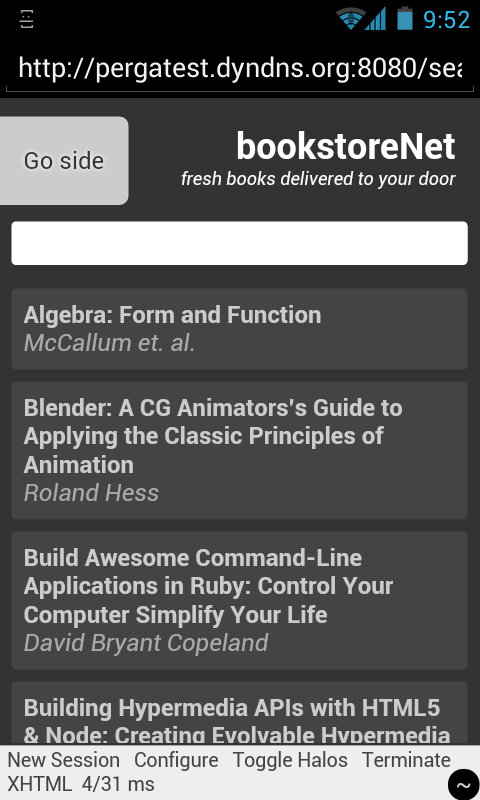
\includegraphics[width=0.3\linewidth]{Screenshots/Screenshot_2013-06-29-09-52-48}
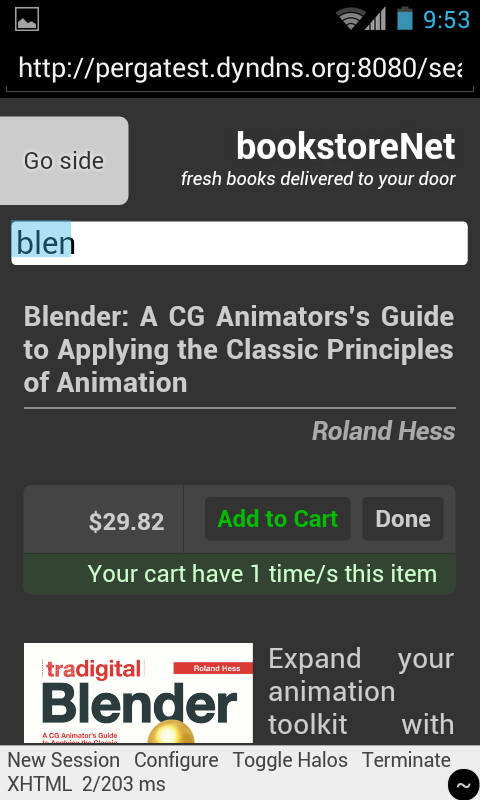
\includegraphics[width=0.3\linewidth]{Screenshots/Screenshot_2013-06-29-09-54-00}
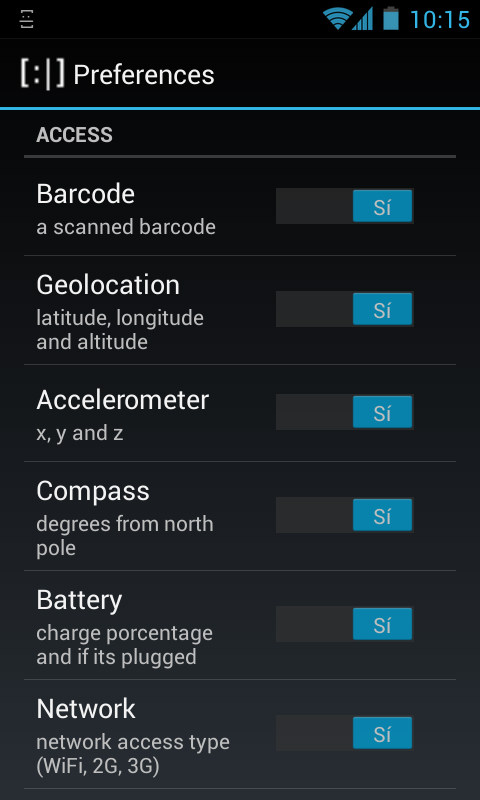
\includegraphics[width=0.3\linewidth]{Screenshots/Screenshot_2013-06-29-10-15-39}
\end{figure}

\clearpage

En el mas \textbf{restrictivo} de los escenarios, el usuario terminará utilizando una \textbf{aplicación web convencional} en donde no exista sensibilidad al contexto.

\clearpage


\section{Conclusión}

\begin{itemize}
\item Se creo una \textbf{aplicación web basada en continuations que se adapte al contexto}.
\item Se explica la combinación de patrones de diseño: \\ \textbf{Adapter} $\rightarrow$ \textbf{Composite} $\rightarrow$ \textbf{Publish/Subscriber} $\rightarrow$ \textbf{Builder}.
\item Se realizó una breve \textbf{comparación} con otros trabajos.
\end{itemize}

\clearpage


%\section{Trabajo a futuro}

%\begin{itemize}
%\item Análisis de \textbf{performance} (tanto a nivel proceso, como transferencia de datos).
%\item Mejorar Builders para soportar de forma total a la \textbf{lógica difusa}.
%\item Ontologías para la \textbf{autoidentificación de sensores} en un dispositivo.
%\item Mejorar la percepción del usuario en torno a la \textbf{administración del acceso y la información privada}.
%\end{itemize}


%\clearpage


%------------------------------------------------

%\thispagestyle{empty} % No slide header and footer

\bibliographystyle{unsrt}
\bibliography{Bibliography}

\clearpage

%------------------------------------------------

\thispagestyle{empty} % No slide header and footer

\begin{tikzpicture}[remember picture,overlay] % Background box
\node [xshift=\paperwidth/2,yshift=\paperheight/2] at (current page.south west)[rectangle,fill,inner sep=0pt,minimum width=\paperwidth,minimum height=\paperheight/3,top color=mygreen,bottom color=mygreen]{}; % Change the height of the box, its colors and position on the page here
\end{tikzpicture}
% Text within the box
\begin{flushright}
\vspace{0.6cm}
\color{white}\sffamily
{\bfseries\LARGE Preguntas?\par} % Request for questions text
\vfill
\end{flushright}

%----------------------------------------------------------------------------------------

\end{document}